\section{Unconstrained optimization (slides)}
\subsection{Exercise 6/11}
Prove the first and second order optimality conditions using
\begin{align*}
f(x^* + d) - f(x^*) = \nabla f(x*)^T d + \frac{1}{2} d^T \nabla^2 f(x^*)d + \text{o}(||d||^2)
\end{align*}

\textbf{Answer}

\hspace{0.5in} \textit{N1 if $x*$ is a local minimum and $f\in \mathcal{C}^1$, then $\nabla f(x^*) = 0$}

If $\nabla f(x^*) = 0$ then $\frac{1}{2} d^T \nabla^2 f(x^*)d = 0$ thus we only consider
\[
f(x^* + d) - f(x^*) = \nabla f(x*)^T d + \text{o}(||d||^2)
\]
Supposing that $\text{o}(||d||^2)$ can be neglected we can rearrange the equation into
\[
\frac{f(x^* + d) - f(x^*)}{d} = \nabla f(x*)^T
\]
which is close to the definition of a limit.

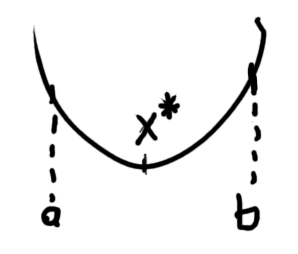
\includegraphics[width=3cm]{fig/unconstrained/6_11.png} For an $x \in [a, b]$ we have $f(x) \geq f(x*)$

\begin{minipage}[t]{.5\textwidth}
  \textbf{From $a$ to $x^*$}\\
  \\
  We have $x < x^*$ and $f(x) - f(x^*) \geq 0$ thus
  \[
  	\frac{f(x) - f(x^*)}{x - x^*} \leq 0
  \]
\end{minipage}
\hspace{0.025\textwidth}\vline\hspace{0.025\textwidth}
\begin{minipage}[t]{.5\textwidth}
  \textbf{From $b$ to $x^*$}\\
  \\
  We have $x > x^*$ and $f(x) - f(x^*) \geq 0$ thus
  \[
  	\frac{f(x) - f(x^*)}{x - x^*} \geq 0
  \]
\end{minipage}

Going back to the definition of a limit we have

\begin{minipage}[t]{.5\textwidth}
  \[
  	\lim_{d\to\infty} \frac{f(x^* + d) - f(x)}{d} \leq 0
  \]
\end{minipage}
\hspace{0.025\textwidth}\vline\hspace{0.025\textwidth}
\begin{minipage}[t]{.5\textwidth}
  \[
  	\lim_{d\to\infty} \frac{f(x^* + d) - f(x)}{d} \geq 0
  \]
\end{minipage}
\\
\\

\hspace{0.5in} \textit{N2 if $x^*$ is a local minimum and $f \in \mathcal{C}^2$, then $\nabla f(x^*) = 0$ and $\nabla^2 f(x^*) = 0$}

If $f \in \mathcal{C}^2$ then $f \in \mathcal{C}^1$ is also true, thus the previous results apply.

\incomplete

\subsection{Exercise 10/71 - Unconstrained optimization with a quadratic objective}
In S2, show that $s^*$ is in fact a \textit{global} minimum!

\textbf{Answer}

\hspace{0.5in} S2 if $Hs^* = -g$ and $H \prec 0$ then $s^*$ is a local minimum

Since $q(s)$ is a quadratic, a local minimum $s*$ of $q$ is automatically a global minimum.

\subsection{Exercise 46/71 - Conjugate gradient \textcolor{green}{???}}
Show that conjugate vectors are necessarily linearly independent.

\answer

Proof by contradiction. If $p_i$ is linearly dependant to a $p_j$ then we have
\[
	a_0 p_0 + a_1 p_1 + \ldots + a_n p_n = 0 \hspace{1cm} n \in \mathbb{Z^*}
\]

Where all $a_n$ are non-zero. Multiply by A
\[
	a_i p_i^T A= 0
\] 
Take the scalar product with $p_i$
\[
	a_i p_i^T A p_i = 0
\]
We know that $A \succ 0$ which means that $p_i^T A p_i > 0$ thus $a_i = 0$ which is contradictory to a linearly dependant system.

\subsection{Exercise 47/71 - Conjugate gradient}

Explain geometrically why $r_{k+1} \perp r_k$ i.e. $r_{k+1}^T r_k = 0$

\answer

When doing a linesearch we stop at a point where the direction is minimal. This also means we are tangent to the contour line (level curve), thus the next direction is orthogonal to the current one.

\begin{center}
	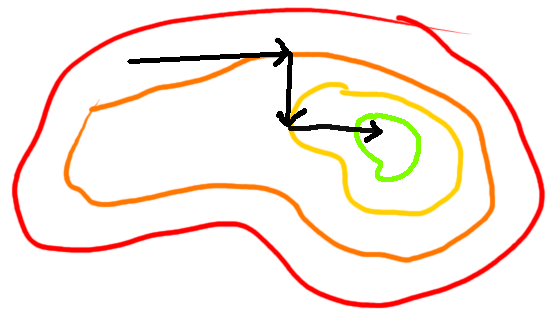
\includegraphics[width=5cm]{fig/unconstrained/47_71.png}
\end{center}


\subsection{Exercise 47/71 - Conjugate gradient}

Find a recurrence to update $q(x_k)$ in the conjugate gradient algorithm.

\answer

Should be something like 
\[
	q(x_{k+1}) = q(x_k) + \nabla q(x_k) \alpha_k A p_k
\]
So the current value of $q$ plus the change in $q$ and how much of that change.

\incomplete

\subsection{Exercice 48/71 - Conjugate gradient}
Prove $A \succ 0$ if and only if $p_k^T A p_k > 0$ for all $k = 0,\ \ldots,\ n-1$

\answer

We know that $A \succ 0$ if all the eigen values $\lambda$ of $A$ are positive and
\[
	A \textbf{v} = \lambda \textbf{v}
\]
so we can rewrite the expression as
\begin{align*}
	p_k^T A p_k = p_k^T \lambda p_k &> 0 \\
	\lambda p_k^T p_k &> 0 \\
	\lambda \| p_k \|^2 &> 0 
\end{align*}
Since $\| p_k \|^2$ must be positive then $\lambda$ must also be positive. Therefore $A \succ 0$.











